\documentclass[hyperref]{ctexart}
\usepackage[left=1.50cm, right=1.50cm, top=2.50cm, bottom=2.50cm]{geometry} %页边距
\usepackage{helvet}
\usepackage{amsmath, amsfonts, amssymb} % 数学公式、符号
\usepackage{mathrsfs}
\usepackage[english]{babel}
\usepackage{graphicx}   % 图片
\usepackage{url}        % 超链接
%\usepackage{bm}         % 加粗方程字体
\usepackage{subfigure}
\usepackage{subcaption}
\usepackage{cleveref}
\usepackage{multirow}
\usepackage{booktabs}
\usepackage{algorithm}
\usepackage{caption}
\usepackage{algorithmic}
\usepackage{graphicx}
\usepackage{subfigure}
\usepackage{float}
\renewcommand{\algorithmicrequire}{ \textbf{Input:}}       
\renewcommand{\algorithmicensure}{ \textbf{Initialize:}} 
\renewcommand{\algorithmicreturn}{ \textbf{Output:}}   
\usepackage{tabularx}    
%算法格式
\usepackage{fancyhdr} %设置页眉、页脚的包
\pagestyle{fancy}
\lhead{}
\chead{}
\lfoot{}
\cfoot{}
\rfoot{}
\usepackage{hyperref} %bookmarks
\hypersetup{colorlinks, bookmarks, unicode} %unicode
\usepackage{multicol}
\title{\textbf{A new optimization model for elliptical artifact reduction in CT using ETV}} %此处用于论文标题
\author{\sffamily author1$^1$, \sffamily author2$^2$, \sffamily author3$^3$}
\date{(Dated: March 16, 2021)} %用于论文的日期
\begin{document}\small
	\maketitle
	\noindent{\bf Abstract: }Elliptical artifacts in cone beam computed tomography (CBCT) images are caused by pixel gain variations using flat-panel detectors or cylindrical metal object(Cross-section is elliptical cylinder), and may lead to structured non-uniformities and deterioration of image quality. The purpose of this study is to propose a method of general Elliptical artifact removal in CBCT images. In this paper, we model the removal of elliptical artifacts as a problem of energy minimization based on the idea of directional total variation and propose a new variational direction based on geometric characteristics of ellipse artifacts. The variational model has been constructed according to the analysis of the edge characteristics of elliptical artifacts. On the one hand, we design a more suitable gradient rotation matrix based on the geometrical characteristics of elliptical artifacts to reduce influences on the structural information of images. On the other hand, we propose model based on the combination of the gradient operator $\nabla$ ,rotation matrix $R$ and the weighted matrix $\lambda$ into the L1-norm regularized term. In order to cope with this nonsmooth model, we employ the alternating direction method of multipliers (ADMM) to solve it. We use~~~\\  %摘要
	
	\noindent{\bf Keywords: DTV; ETV; ADMM; elliptical; artifact; CT... %关键词摘要
	\begin{multicols}{2}
		\section{Introduction}
		Flat-panel detectors can acquire 2D projections using x-rays (Cho et  al 1995, Scarfe et  al 2006), and have been widely used in cone-beam CT (CBCT) systems. In addition, flat-panel detectors can be used in many fields such as biomedical imaging, image-guided radiotherapy (IGRT) (Jaffray et al 2002, Yan et al 2014, Liang et al 2016), industrial x-ray flaw detection (Hofmann et al 2004, Zhang et al 2005), and materials research. However, some ring artifacts are always located at the center of the rotation axis in the reconstructed images, mainly due to the pixel gain variations in the detector (Vidal et al 2005). They appear in the form of concentric rings in the reconstructed image. In this paper, we consider the removal of ellipse artifacts. On the one hand, the ring is also a special ellipse, so our model is still efficient in removing ring artifacts. On the other hand, ring artifacts may turn into elliptical due to the deviation of CT reconstruction, and the effect of traditional ring artifact removal methods will deteriorate in this case, so we propose the model of elliptical artifacts reduction.
		The artifacts severely impair the quantification of the diagnosis. In addition, these artifacts are considered an integral part of the image (e.g. tumor) by the computer, which may lead to a wrong diagnosis (Davis and Elliott 1997, Sadi et al 2010). In radiotherapy, severe artifacts may be identified as bone, resulting in incorrect positioning. Since these artifacts make post-processing and quantitative evaluation complicated, the development of an effective and convincing method of elliptical artifact removal is crucial.
		In recent years, many researchers have been developing CBCT methods for ring artifact 
		removal (Raven 1998, Tang et al 1999, Boin and Haibel 2006, Ketcham 2006, Sadi et al 2010, 
		Wu et al 2015a). These methods can be roughly divided into two categories: pre-processing in the projection domain and post-processing in the image domain. Pre-processing in the projection domain needs to access the raw projection data, which restricts the applicability of the algorithm. Thus, a post-processing method which was inde-pendent of the raw data was proposed in order to significantly extend the range of application. A most popular post-processing method for removing ring artifacts is transforming the reconstructed image from a Cartesian to polar coordinate system (Chen et al 2010, Wei et al 2013). Here, the ring artifacts are manifest as stripe artifacts in polar coordinate systems and, after image processing in polar coordinates, the image is transformed back into a Cartesian coordinate system. In 2004, Jan Sijbers et al (Sijbers and Postnovz 2004) proposed a ring artifact correction method based on morphological operators. First, a region of interest (ROI) to be processed is selected. Then a sliding window is applied to generate the artifact template and acquire the corrected image by subtraction. The parameter selection is crucial to the accuracy of the artifact correction in this method. Subsequently, in 2009, Chen et al (2009) presented an effective method using independent component analysis (ICA), but this process deteriorates the image details. Kyriakou et al (2009) and Prell et al (2009) have used a median filter to remove stripe artifacts in polar coordinates with the assumption that the gray value feature in the ring artifacts are local extrema. Recently, Yan et al (2016) proposed a method of variationbased ring artifact removal with sparse constraint; this method showed effective correction, but the process of coordinate transformation deteriorated the spatial resolution of the images. 
		However, the ellipse is a sinusoidal image in polar coordinates, which has a high degree of similarity with the CT image itself, so it cannot be processed by the polar coordinate transformation method. Here we analyze the geometric characteristics of the ellipse artifact and propose a new variational model has been constructed according to the analysis of the mechanism and characteristics of elliptical artifacts.
		How to evalucate it~~~~~~
		
		\section{MATERICALS AND METHODS}
		\subsection{Directional total variation}
		The DTV was first proposed by Bayram and Kamasak in 2012. It can be defined as
		\begin{flalign}
			\begin{split}
				TV_{\alpha,\theta}(f)=\mathop{sup}_{v(i,j)\in E_{\alpha,\theta}} \quad \left \langle \nabla f , v\right \rangle
			\end{split}
		\end{flalign}
	
		where:
		\begin{equation}
			\begin{split}
				v(i,j) = \begin{bmatrix} v_1(i,j) \\  v_2(i,j)  \end{bmatrix},\nabla f (i,j) = \begin{pmatrix} \nabla_1 f(i,j) \\ \nabla_2 f(i,j)  \end{pmatrix}
			\end{split}
		\end{equation}
		\begin{equation}
			\begin{split}
				\nabla_1 f(i,j) =  f(i,j)-f(i-1,j) \\ \nabla_2 f(i,j) = f(i,j)-f(i,j-1) 
			\end{split}
		\end{equation}
	
		$E_{\alpha,\theta}$  is an ellipse aligned along the angle $\theta$ with the semi-minor axis and semi-major axis of 1 and $\alpha > 1$. $v(i,j)$ is taken on the ellipse  $E_{\alpha,\theta}$ and $\nabla_1f(i,j)$, $\nabla_2f(i,j) $ are the vertical and horizontal differeces for the pixel $(i,j)$ in the 2D image $X$, respectively.So The pseudo norm defined by (1) is more senstive to variations along the major axis.Also note that $\theta$ in $RTV_{\alpha,\theta}$ is a matrix which is a function of the coordinate $(i,j)$ of the image X.
		\subsection{Elliptical total variation}
		When the semi-major axis of the ellipse is along a specific direction, the dominant structures along this direction are preserved. In the elliptial artifact reduction application, however, not noly the directions of the elliptical artifacts change, we would also like to penalize the elliptical structures. As a result, we propose the following DTV-based regularization named elliptical total variation( $E_{\beta,\lambda}$) in this paper. In order to penalize the elliptical artifacts. We suggest placing the semi-minor axis of the ellipses along with the tangential vector of the elliptical artifacts. Thus,  neighbor pixels along the normal directions are utilzed with higher weights than other neighboring pixels.
		
		It's possible to obtain ETV by replacing $\theta$ in(1) with normal directions of elliptical artifacts. In particular, a special transform of rotation matries can contribute to increase the sensitivity to changes towards certain directions of different pixel in elliptical artifacts.
		
		Supposed that $\beta$ is a function of the coordinate $(i,j)$ of image. Standart equation for ellipse(supposed the semi-major axis is along the $y$-axis):
		\begin{equation}
			\begin{split}
				\frac{x^2}{b^2} + \frac{y^2}{a^2} = 1
			\end{split}
		\end{equation}
		
		By deriving x, we can easily get the function of $\alpha$ :
		\begin{figure}[H]
			\centering
			\subfigure[LFR]{
				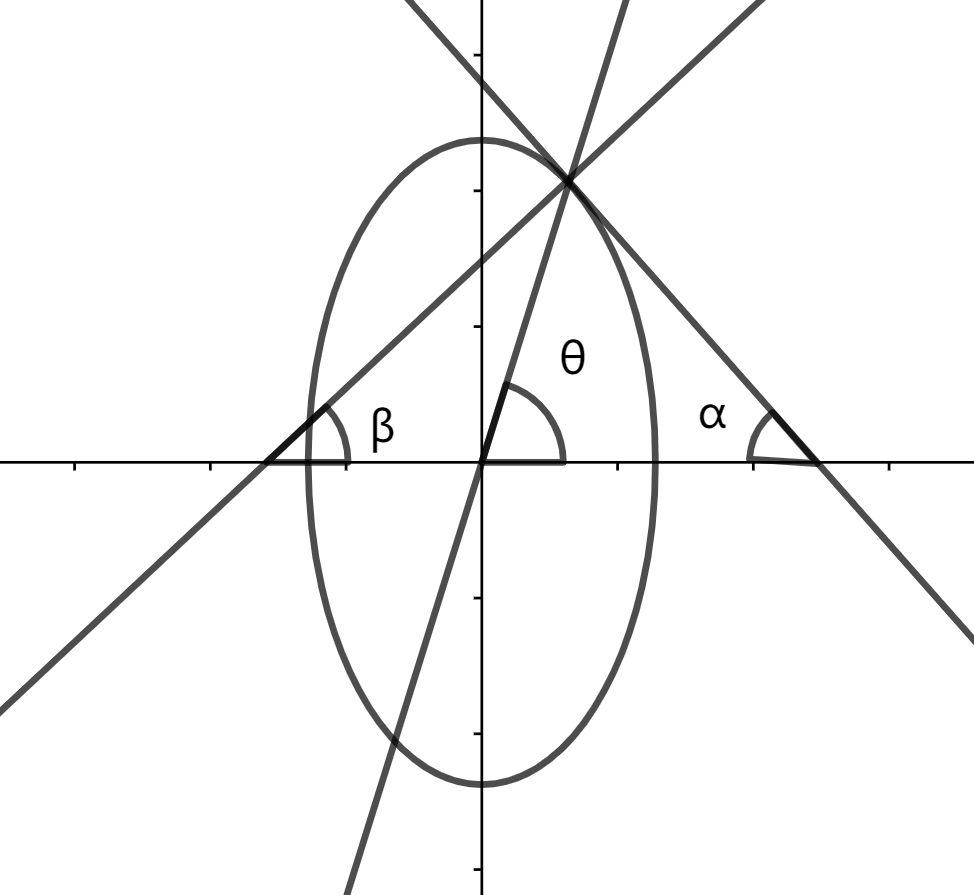
\includegraphics[scale=0.3]{椭圆.png}
				\label{fig1}
			}
		\end{figure}
		\begin{equation}
			\begin{split}
				tan\alpha  = \frac{dy}{dx} = - \frac{a^2 x}{b^2 y}
			\end{split}
		\end{equation}
		$\alpha$ and $\beta$ are complementary, so
		\begin{equation}
			\begin{split}
				\beta  =arctan(-\frac{b^2y}{a^2x})
			\end{split}
		\end{equation}
	
		Acording to Bayram and Kamasak let $R_\beta$ and $\Lambda_\lambda$ denote the rotation and scaling matrices respectively as:
		\begin{equation}
			\begin{split}
				R_{\beta} = \begin{bmatrix} cos\beta & sin\beta \\- sin\beta & cos\beta \end{bmatrix},\Lambda_{\lambda} = \begin{bmatrix} \lambda_1 & 0 \\ 0 & 1 \end{bmatrix}
			\end{split}
		\end{equation}
		Note that $E_{\lambda,\beta}$ and $B_2$ are related as $E_{\lambda,\beta} = R_\beta \Lambda_\lambda B_2$.Furthermore, let us now define the operators $R_\beta $, $\Lambda_\lambda$, that act on the vector fields as $(R_\beta v)(i,j) = R_\beta(v(i,j))$ and $(\Lambda_\lambda)(i,j) = \Lambda_\lambda(v(i,j))$. Using the fact that $R^T_\beta = R_{-\beta}$ and $\Lambda^T_\lambda = \Lambda_\lambda,ETV_{\lambda, \beta}$ can be expressed in the following forms:
		\begin{equation}
			\begin{split}
				ETV_{\beta,\lambda}(f)& =\mathop{sup}_{v(i,j)\in R_{\beta}\Lambda_{\lambda}B_2} \left \langle \nabla f,v \right \rangle \\
				& =\mathop{sup}_{v(i,j)\in B_2} \left \langle \nabla f,R_{\beta}\Lambda_{\lambda},v \right \rangle \\
				& =\mathop{sup}_{v(i,j)\in B_2} \left \langle \Lambda_\lambda R_{-\beta}\nabla f,v \right \rangle \\
			\end{split}
		\end{equation}
		
		Where:
		\begin{equation}
			\begin{split}
				\beta = arctan(-\frac{b^2 y}{a^2 x})
			\end{split}
		\end{equation}
		Therefore, the optimization problem also proposed as:
		\begin{equation}
			\begin{split}
				\min \frac{\lambda}{2} \Vert y-f\Vert_2^2 +  \Vert T \nabla f\Vert_{2,1}
			\end{split}
		\end{equation}
		where the term $\Vert y-f\Vert_2^2$ makes the input and result not deviate wildly. The effect of removing elliptical artifact in CT is introduced by a new regularizer $\Vert T \nabla f\Vert_{2,1}$,where rotation and scaling matrices are efficiently coupled as $T$, expressed as $T=\Lambda_\lambda R_{-\beta}$
		
		\subsection{Methodology}
			In order to use the ADMM, we need to firstly transform the proposed model(2) into the following constrained optimization problem
			\begin{equation}\left\{
				\begin{split}
					& \mathop{\min}_{w,v,u} \frac{\lambda}{2}\Vert f-y \Vert_{2}^{2} + \Vert w \Vert_{2,1} \\
					& s.t. \, \, \, w:=(w_1,w_2)^T = Tv \, and \, v:=(v_!,v_2)^T = \nabla u
				\end{split}
				\right.
			\end{equation}
			The aim of this transformation is to move out two linear operators $\nabla$ and $T$ from the $l^1$ -norm in order to use some efficient numerical methods. Then, based on the augmented Lagrange (AL) method, we rewrite the  problem (11) as the saddle-point problem
			\begin{equation}
				\begin{split}
					 \mathop{\min}_{w,v,u} \, \mathop{\max}_{\alpha,\beta} \mathscr{L}= & \frac{\lambda}{2}\Vert f-y \Vert_{2}^{2} +	\left \langle \alpha,v - \nabla u \right \rangle + \frac{\gamma_1}{2}\Vert v-\nabla u  \Vert_{2}^{2} \\
					 &+\Vert w \Vert_{2,1} + \langle \beta,w - Tv  \rangle + \frac{\gamma_2}{2}\Vert w-Tv \Vert_{2}^{2} 
				\end{split}
			\end{equation}
		where $\gamma_1>0,\gamma_2>0$ are the penalty parameters and $\alpha = (\alpha_1,\alpha_2)>0,\beta = (\beta_1,\beta_2)>0$ are the Lagrange multipliers (i.e.,dual variables) responding to the splitting variables $w$ and $v$ ,respectively. In the problem(14),it includes five subvaribles, so we need to solve one of subvariables and simultaneously fix others when using the ADMM as:
		 
		\begin{tabular}{l}
			\hline
			$Algorithm 1: ADMM to solve the problem $\\
		\hline
			1.Initialize: $\lambda$ > 0  and choose original value of  $u^0 , v^0,\alpha ^0 and,\beta^0 $ \\
			2.For k=1,2,...,  obtaining  $(u^{k+1}, v^{k+1}, w^{k+1})by$ \\
			3.End for until stopping rule meets;\\ 
			4.Set $u:= u^{k+1}$ as the denoising image.\\
			\hline
		\end{tabular}
		In the following, we consider how to solve subproblems (15) (a)-(c).
		
		- For the subproblem (15)(a), it is the classic $l^2 - l^1$  problem as 
		\begin{equation}
			\begin{split}
				w^{k+1} :=  \mathop{\arg \min}_{w}  \frac{\gamma_2}{2} \left \Vert w- \left( Tv^k - \frac{\beta^k}{\gamma_2}\right)  \right \Vert^2_2 + \Vert w \Vert_{2,1}
			\end{split}
		\end{equation}
		By using the soft-thresholding operator (5), its closed-form solution can be written as
		\begin{equation}
			\begin{split}
				w^{k+1} :=  Prox \Vert . \Vert_{2,1}\left( \left \Vert  Tv^k - \frac{\beta^k}{\gamma_2}  \right \Vert , \gamma_2 \right) 
			\end{split}
		\end{equation}
	
		- For the subproblem (15)(b), it is a smoothing optimization problem. So its optimal 	solution $v^{k+1}$ satisfies the following linear system
		
		\begin{equation}\left\{
			\begin{split}
				& a^k_1 + \gamma_1(v_1^{k+1} - \nabla_x f^k) - t_1\beta^{k+1} + \gamma_2 t_1(t_1v_1^{k+1}-w_1^{k+1}) = 0\\
				& a^k_1 + \gamma_1(v_2^{k+1} - \nabla_y f^k) - t_2\beta^{k+1} + \gamma_2 t_2(t_2v_2^{k+1}-w_2^{k+1}) = 0
			\end{split}
			\right.
		\end{equation}

			
		With a simple computation, its explicit solution can be obtained by
		
		\begin{equation}\left\{
			\begin{split}
				& v_1^{k+1} = \frac{\gamma_1 \nabla_x f^k + t_1\beta_1^k  + \gamma_2 t_1 w_1 ^{k+1} - \alpha_1^k}{\gamma_1 + \gamma_2 t_1^2}\\
				& v_1^{k+1} = \frac{\gamma_1 \nabla_y f^k + t_2\beta_2^k  + \gamma_2 t_2 w_2 ^{k+1} - \alpha_2^k}{\gamma_1 + \gamma_2 t_1^2}
			\end{split}
			\right.
		\end{equation}
		
		- For the subproblem (15)(C), it is a least squares optimal problem and the corresponding 	Euler-Lagrange equation is
		
		\begin{equation}
			\begin{split}
				(\lambda I- \gamma_1 \nabla)u^{k+1} = \lambda y - div a^{k+1} - \gamma_1 div v^{k+1 }
			\end{split}
		\end{equation}
		
		
		For this linear equation system, different boundary conditions lead to different numerical methods. In fact, we shall notice that the Laplacian operator $-\Delta$ is positive semi-definite when using the zero Neumann boundary condition or the zero Dirichlet boundary condition. In this case, we can use the preconditioned conjugate gradient (PCG) method [40] to solve it since $\lambda$ and $\gamma_1$ are both positive scalars, the matrix on the left-hand-side of the above system is symmetric and positive definite. However here we assume that the boundary condition is periodic, so the problem (19) can be efficiently solved by
		
		\begin{equation}
			\begin{split}
				f^{k+1}  = F^{-1}\left(  \frac{	 \lambda F(y) - F(div a^{k}) - \gamma_1 F(div v^{k+1})}{\lambda F(I) - \gamma_1 F(\Delta)} \right) 
			\end{split}
		\end{equation}
		
		where $F(.)$ and $F{-1}1$(.) are the fast Fourier transformation (FFT) and the inverse transformation, respectively.
		
		\section{实验结果与分析}
		In this section, the proposed method is evaluated using both simulated and real datasets to evaluate the performance of the proposed model (ETV) and the numerical method. All experiments are performed via using MATLAB (R2020a) on a windows10 (64bit) desktop computer with an Inter Core i5-7300QH、2. 50 GHz processor andon the comparisons between the ATV (2) and other TV-based models such as the ROF 8.0GB of RAM. 
		
		\subsection{模拟数据实验}
		In this subsection,We consider using Sepp-Logan phantom and Lena phantom to evaluate the ETV。我们采用一些常用的定量评估方法来评价去除伪影后的图像效果, 在此引入两种常用的图像评价指标: 峰值信噪比(Peak signal-to-noise ratio, PSNR) 和平均结构相似性 (Mean structural similarity, MSSIM). PSNR是最普遍和使用最为广泛的一种图像质量评价指标,是基于对应像素点间的误差, 将处理结果与参考图像的像素值进行比较, 处理结果的 PSNR 值越大说明与参考图像的像素值差异越小, 即算法性能越好.MSSIM 是一种更接近于人类视觉的图像质量评测方法, 指标值体现了处理结果与参考图像间的亮度、对比度以及结构的相似性, 更多地与图像视觉特征相关, 值越大说明处理结果视觉上越接近理想的参考图像.In order to evaluate the performance of the proposed method, simulated-ellipse artifacts were superimposed on the Lena phantom and Shepp-Logan phantom to generate the corrupted images.In order to simulate the difference of artifacts caused by different use of machine,We randomly added different shades of artifact.
		
		\subsubsection{Shepp–Logan phantom}
		An equidistant fan-beam geometry is assumed with 512 detector bins each of which has a width of 0.11 mm. The number of view angles is 640. The reconstructed image includes 512 * 512 pixels each of which covers an area of 0.05 * 0.05 mm2. Seventy of 512 detector bins are randomly selected and added with a 70 * 1 vector of normally distributed random number to mimic the corrupted detector bins. The standard deviation is 0.01.
		
		
	\end{multicols}
	
			\begin{figure}[htbp]
				\centering
				\subfigure[pic1.]{
					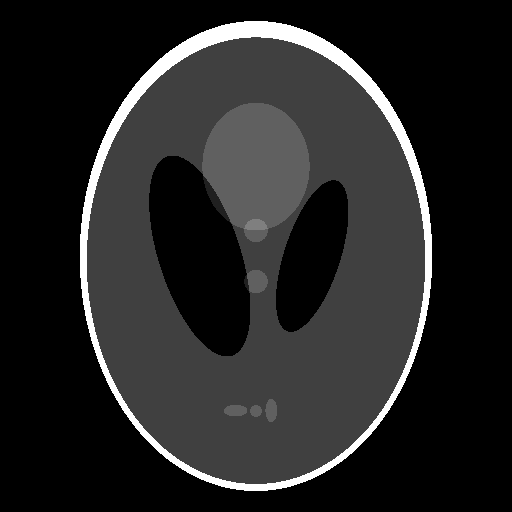
\includegraphics[scale=0.2]{C:\Users\jinzong53\Desktop\CT论文\论文\sigma0.01-Shepp-Logan\O.png}
				}
				\quad
				\subfigure[pic2.]{
					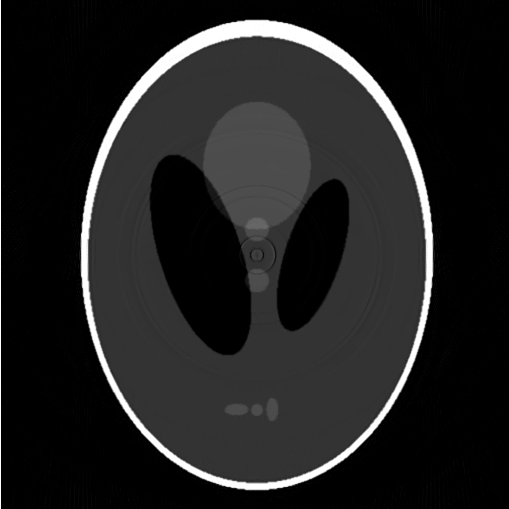
\includegraphics[scale=0.2]{ETV.png}
				}
				\quad
				\subfigure[pic3.]{
					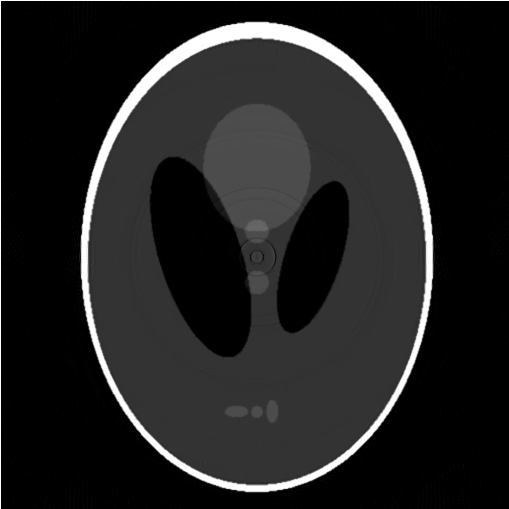
\includegraphics[scale=0.2]{RTV.png}
				}
				\quad
				\subfigure[pic4.]{
					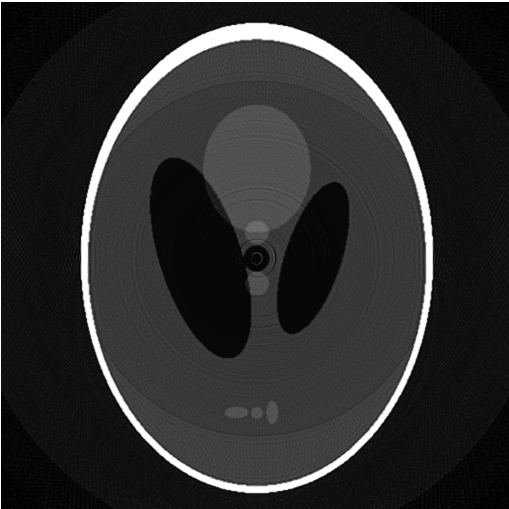
\includegraphics[scale=0.2]{ringREM.png}
				}
				\caption{Results of Shepp–Logan phantom (display window: [0 1.0])}
			\end{figure}
		
			\begin{multicols}{2}
		
		
		 Figure * displays the original and the reconstructed Shepp–Logan phantom containing the rings (which is referred as the corrupted image) along with the reconstructed phantoms using the ring artifact reduction methods RRRTV and RINGREM and our ETV algorithm. By an over-view on this figure, the method RRRTV and our ETV algorithm are perfectly able to remove the ring artifacts. In Fig. 5, the absolute values of the difference of the reconstructed images with respect to the original phantom are displayed. Since the absolute value is used, the display window starts from zero, and darker regions indicate better ring removal and reconstruction result. It can be seen that the difference images obtained from our algorithm are darker as a whole compared to other competing methods.It can be seen that only our algorithm and the method by RRRTV were able to remove all the ring artifacts and ringREM have difficulties in removing the rings especially around the center. 
		
		\begin{tabular}{ccc}
			\hline
			\multirow{2}{*}{算法} & \multicolumn{2}{c}{Shepp-Logan 图像}  \\
			& SSIM             & PSNR                 \\ \hline
			ETV                  & 0.9564                & 78.3933                 \\
			RTV                 & 0.9623                & 78.4835                \\
			RINGREM               & 0.6173                & 27.6739                   \\ \hline
		\end{tabular}
		\end{multicols}
	
		
		\begin{figure}[htbp]
			\centering
			\subfigure[pic1.]{
				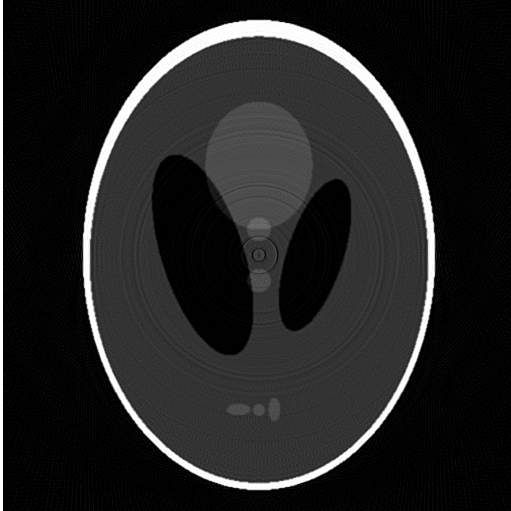
\includegraphics[scale=0.2]{原图.png}
			}
			\quad
			\subfigure[pic2.]{
				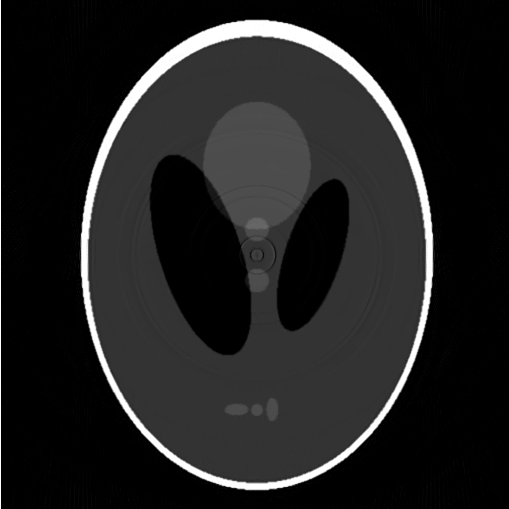
\includegraphics[scale=0.2]{ETV.png}
			}
			\quad
			\subfigure[pic3.]{
				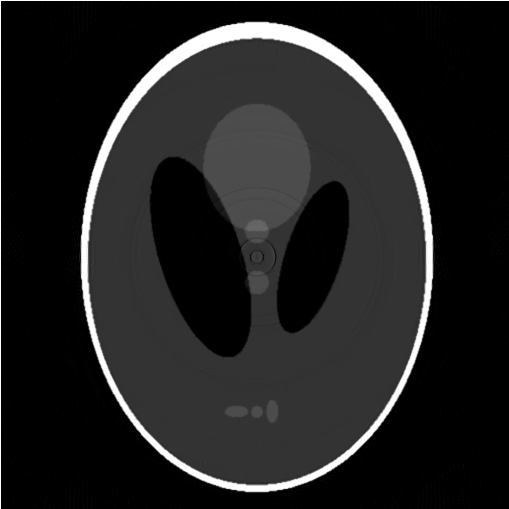
\includegraphics[scale=0.2]{RTV.png}
			}
			\quad
			\subfigure[pic4.]{
				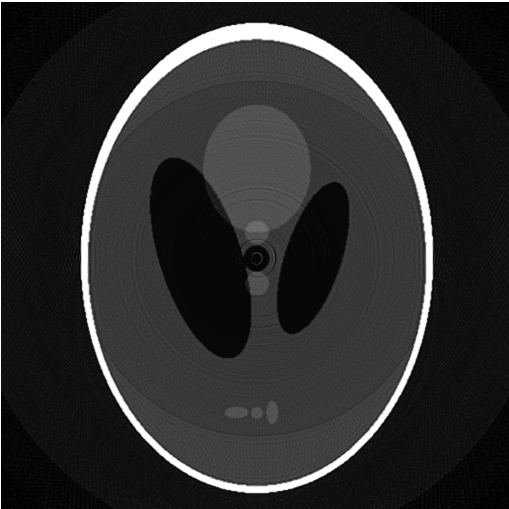
\includegraphics[scale=0.2]{ringREM.png}
			}
			\caption{Results of Shepp–Logan phantom (display window: [0 1.0])}
		\end{figure}
		
		\begin{figure}[htbp]
			\centering
			\subfigure[pic1.]{
				
\includegraphics[scale=0.2]{绝对值-原始.png}
			}
			\quad
			\subfigure[pic2.]{
				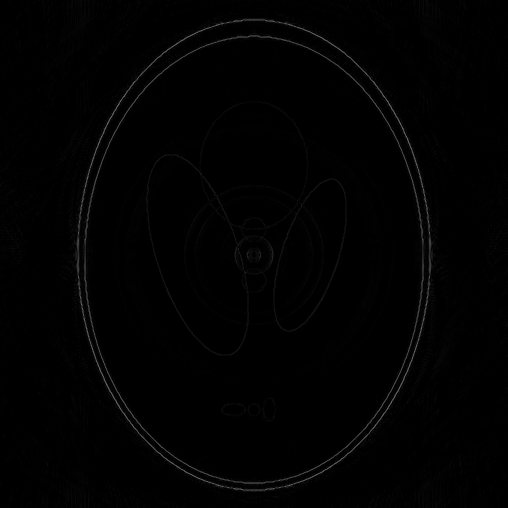
\includegraphics[scale=0.2]{绝对值-ETV.png}
			}
			\quad
			\subfigure[pic3.]{
				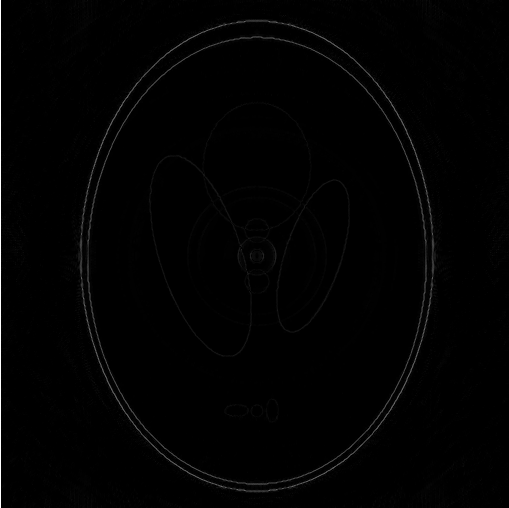
\includegraphics[scale=0.2]{绝对值-RTV.png}
			}
			\quad
			\subfigure[pic4.]{
				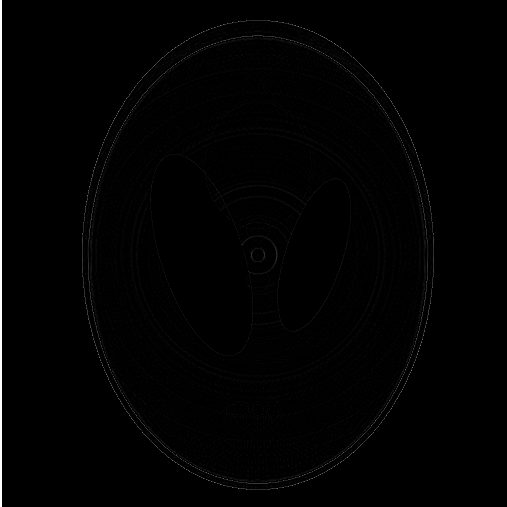
\includegraphics[scale=0.2]{绝对值-ringREM.png}
			}
			\caption{Results of Shepp–Logan phantom (display window: [0 1.0])}
		\end{figure}
		
		\begin{figure}[htbp]
			\centering
			\subfigure[pic1.]{
				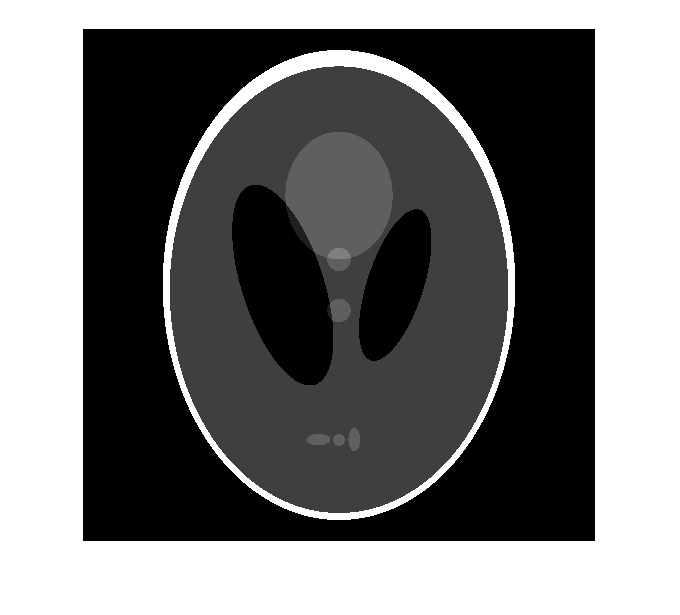
\includegraphics[scale=0.2]{11.png}
				%\caption{fig1}
			}
			\quad
			\subfigure[pic2.]{
				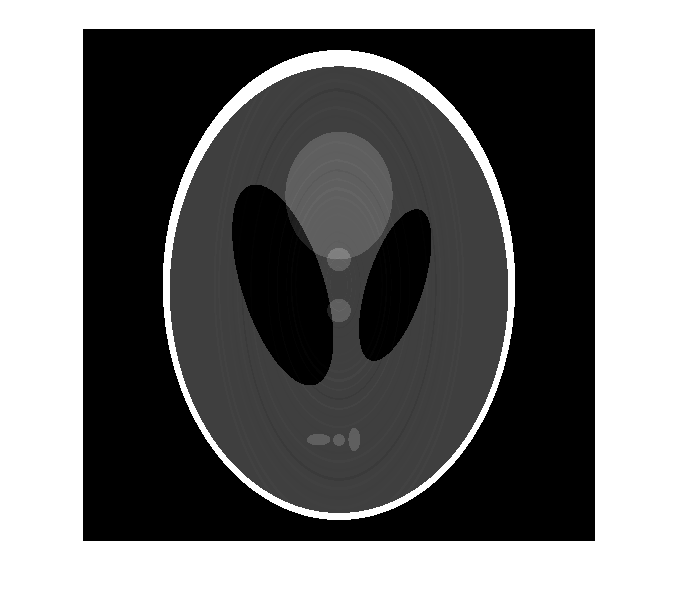
\includegraphics[scale=0.2]{22.png}
			}
			\quad
			\subfigure[pic3.]{
				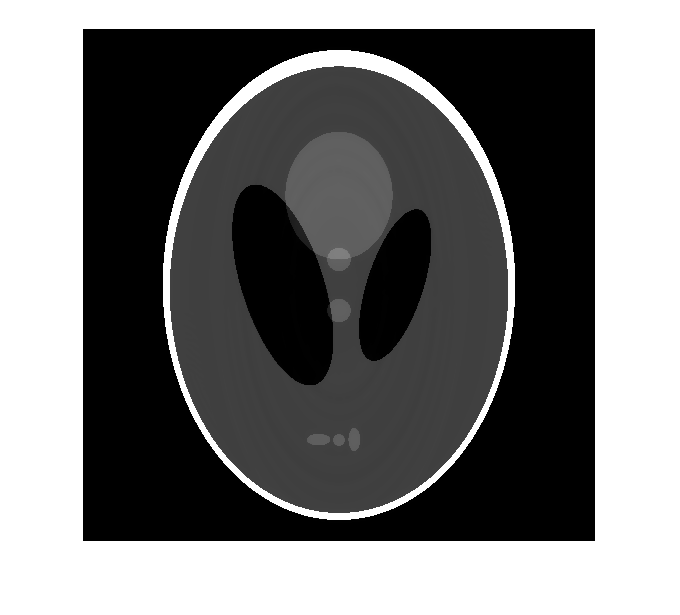
\includegraphics[scale=0.2]{33.png}
			}
			\quad
			\subfigure[pic4.]{
				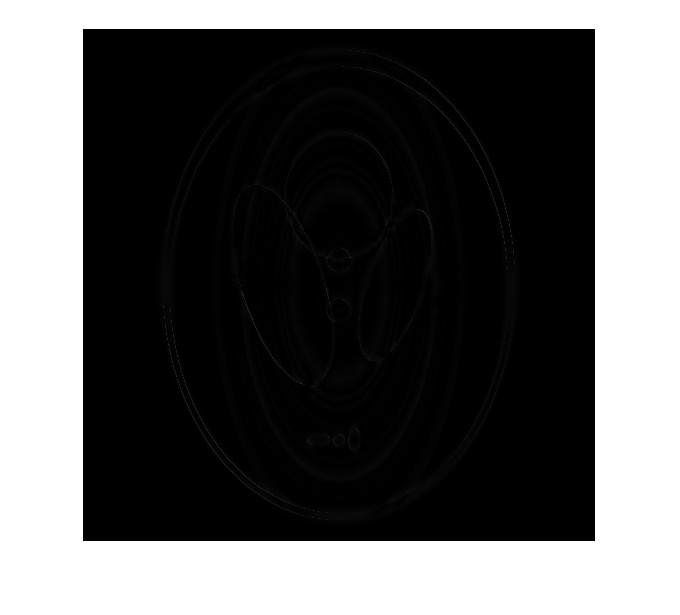
\includegraphics[scale=0.2]{44.png}
			}
			\quad
			\subfigure[pic5.]{
				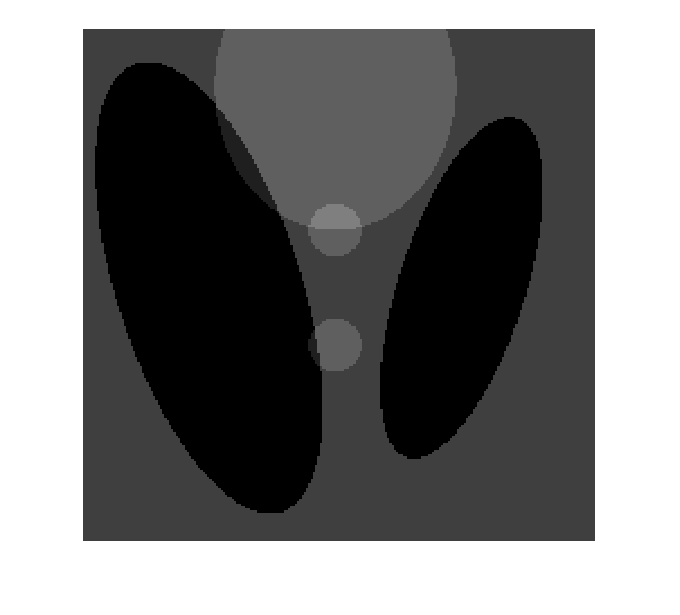
\includegraphics[scale=0.2]{11-1.png}
			}
			\quad
			\subfigure[pic6.]{
				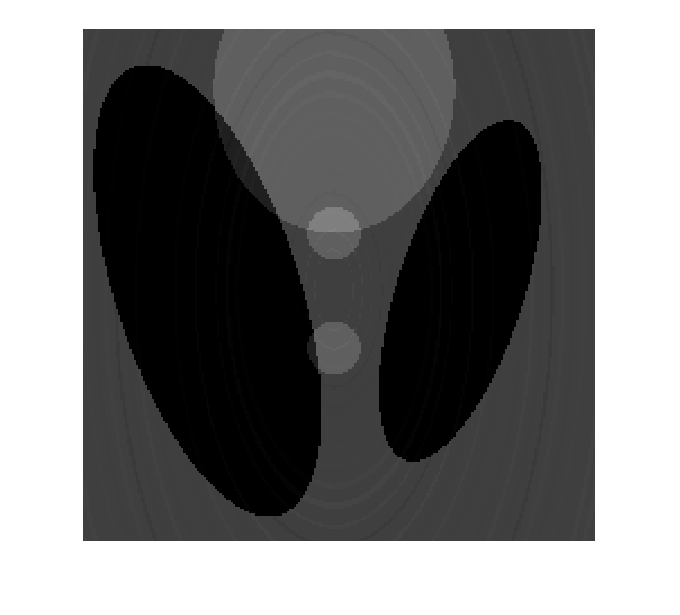
\includegraphics[scale=0.2]{22-1.png}
			}
			\quad
			\subfigure[pic1.]{
				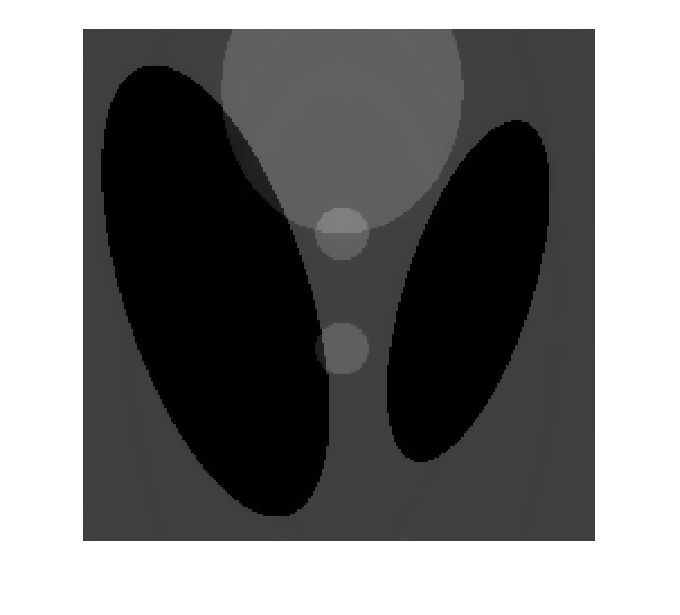
\includegraphics[scale=0.2]{33-1.png}
				%\caption{fig1}
			}
			\quad
			\subfigure[pic2.]{
				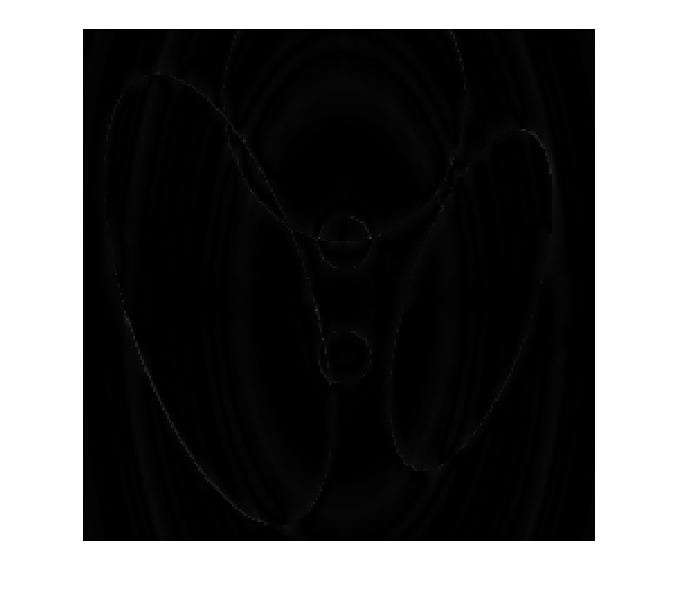
\includegraphics[scale=0.2]{44-1.png}
			}
			\quad
			\subfigure[pic5.]{
				
\includegraphics[scale=0.2]{11-2.png}
			}
			\quad
			\subfigure[pic6.]{
				
\includegraphics[scale=0.2]{22-2.png}
			}
			\quad
			\subfigure[pic1.]{
				
\includegraphics[scale=0.2]{33-2.png}
				%\caption{fig1}
			}
			\quad
			\subfigure[pic2.]{
				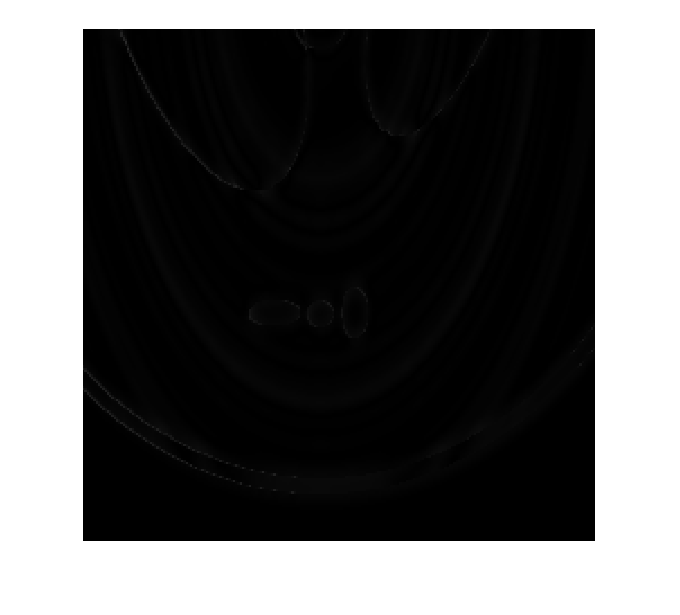
\includegraphics[scale=0.2]{44-2.png}
			}
			\quad
		\end{figure}
	
		\begin{multicols}{2}
		
		Figure * shows the original image, the corrupted image and the processing resulty. (E) ~ (J) is the ROI image of different regions. We use the range of pixel value of the image loss to represent the image generated by the detector with slight loss. It is obvious from (d), (g), (J) that most artifacts have been eliminated within this loss range. We put the ROI in the center part of the image, This part of the artifact is often the most difficult to effectivily removal, from (g), (J) we can see that this part of the artifact is only a little residue. In order to more intuitive image quality from the data, we introduce PSNR and SSIM to judge the image quality. From the table we can see that the algorithm mentioned in this paper has good processing effect for this degree of image damage.
		
		\begin{tabular}{ccc}
			\hline
			\multirow{2}{*}{算法} & \multicolumn{2}{c}{Shepp-Logan 图像}  \\
			& SSIM             & PSNR                 \\ \hline
			1                  & 0.9970                & 50.918                \\
			2                & 0.9980                & 53.457                \\
			3               & 0.9973                & 52.891                   \\ \hline
		\end{tabular}
		\end{multicols}
	
		\begin{figure}[htbp]
			\centering
			\subfigure[pic1.]{
				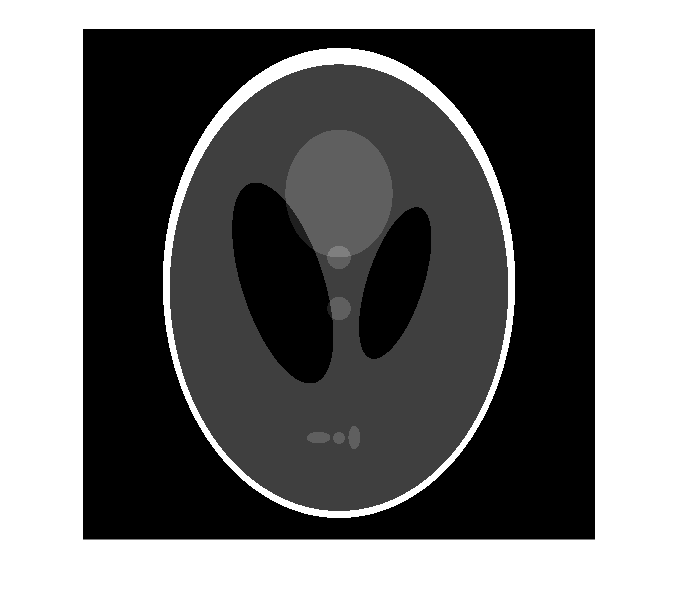
\includegraphics[scale=0.2]{1.png}
				%\caption{fig1}
			}
			\quad
			\subfigure[pic2.]{
				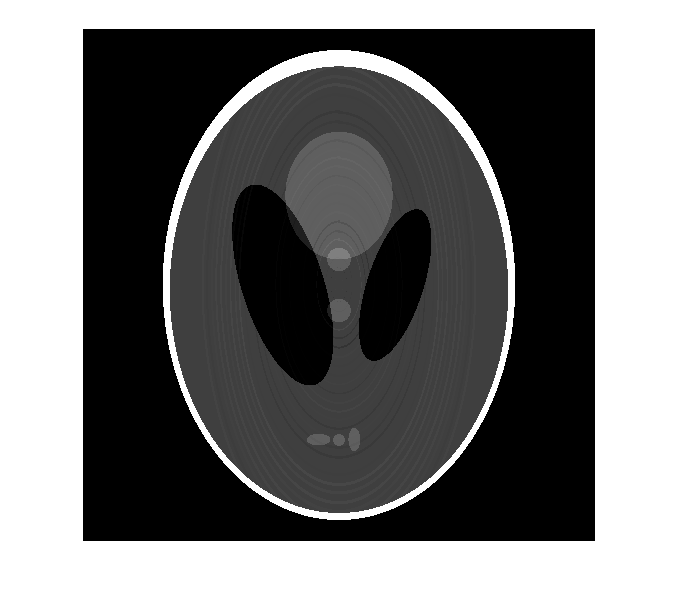
\includegraphics[scale=0.2]{2.png}
			}
			\quad
			\subfigure[pic3.]{
				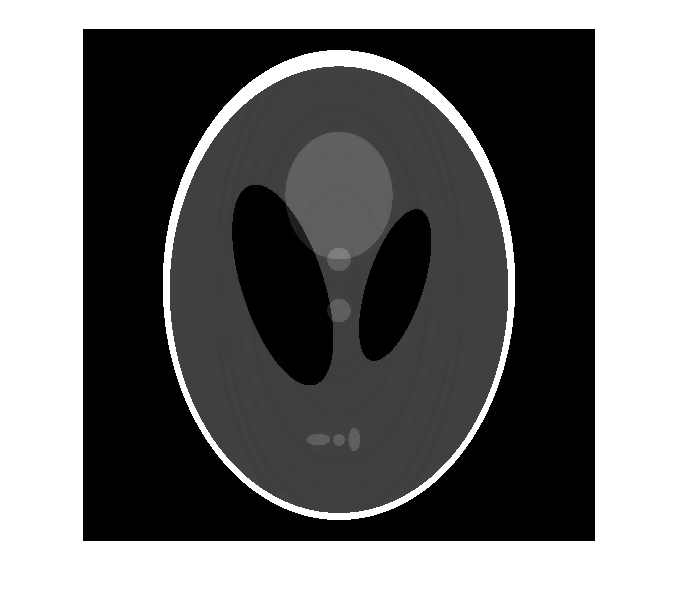
\includegraphics[scale=0.2]{3.png}
			}
			\quad
			\subfigure[pic4.]{
				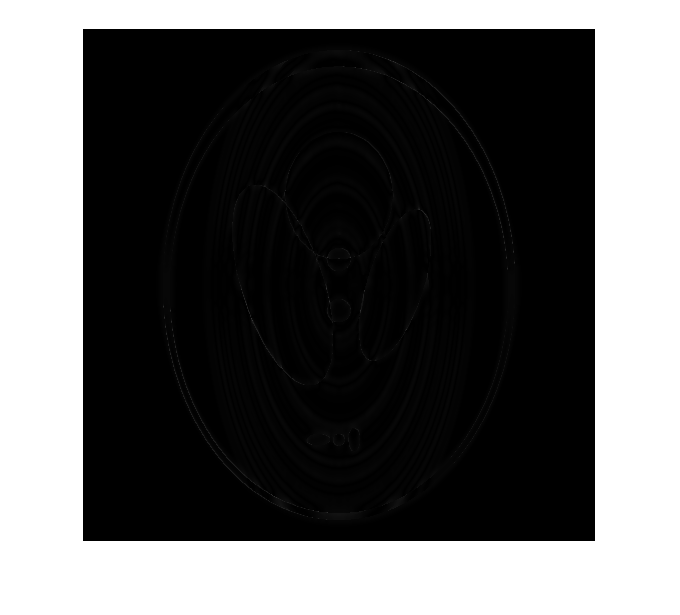
\includegraphics[scale=0.2]{4.png}
			}
			\quad
			\subfigure[pic5.]{
				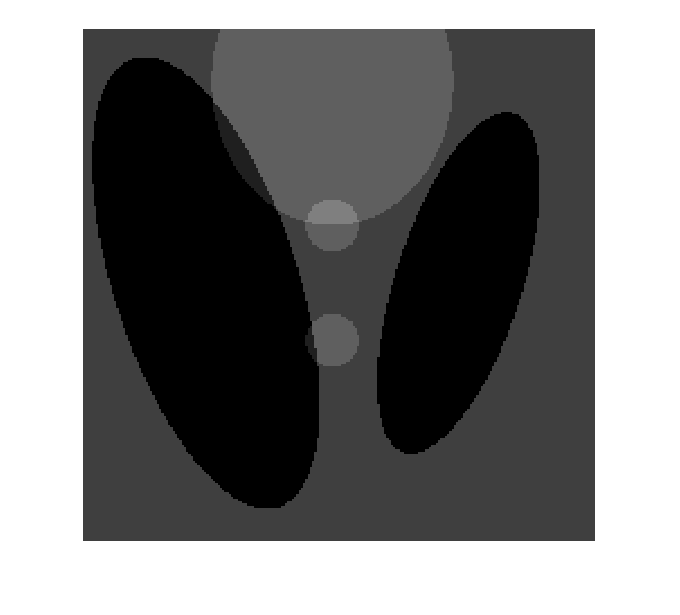
\includegraphics[scale=0.2]{1-1.png}
			}
			\quad
			\subfigure[pic6.]{
				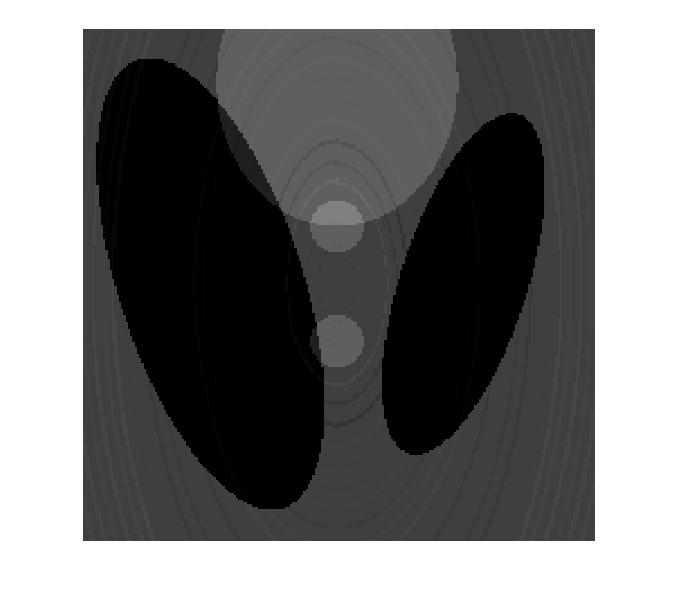
\includegraphics[scale=0.2]{2-1.png}
			}
			\quad
			\subfigure[pic1.]{
				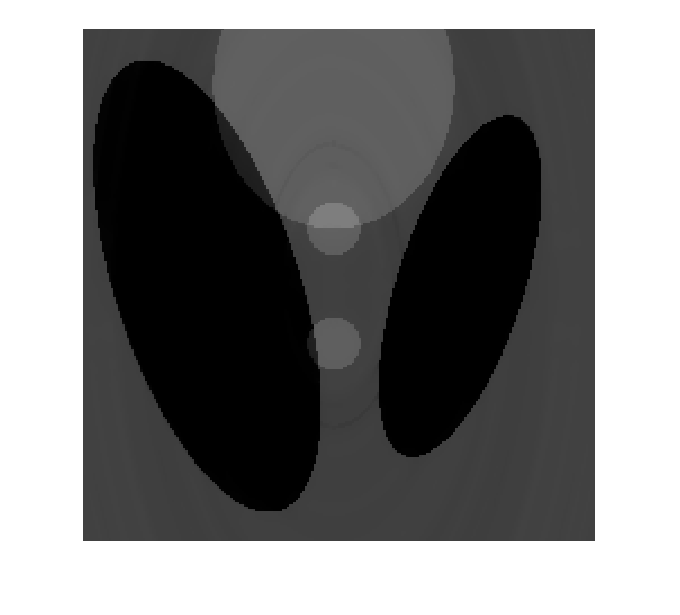
\includegraphics[scale=0.2]{3-1.png}
				%\caption{fig1}
			}
			\quad
			\subfigure[pic2.]{
				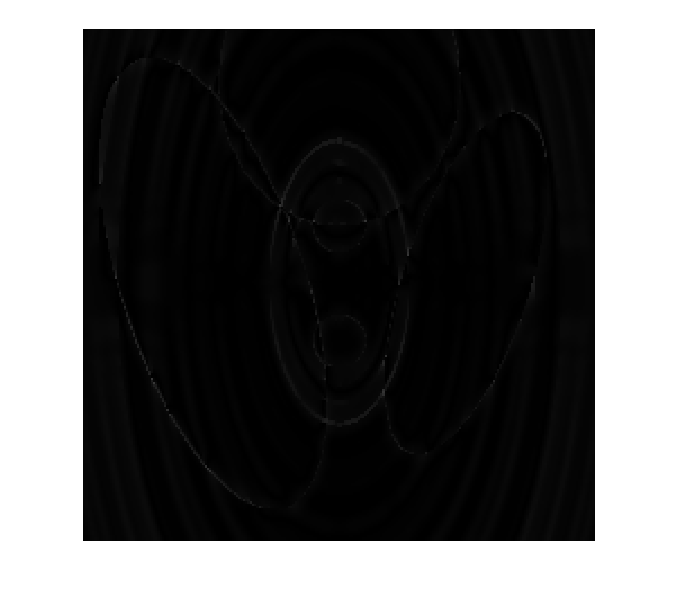
\includegraphics[scale=0.2]{4-1.png}
			}
			\quad
			\subfigure[pic5.]{
				
\includegraphics[scale=0.2]{1-2.png}
			}
			\quad
			\subfigure[pic6.]{
				
\includegraphics[scale=0.2]{2-2.png}
			}
			\quad
			\subfigure[pic1.]{
				
\includegraphics[scale=0.2]{3-2.png}
				%\caption{fig1}
			}
			\quad
			\subfigure[pic2.]{
				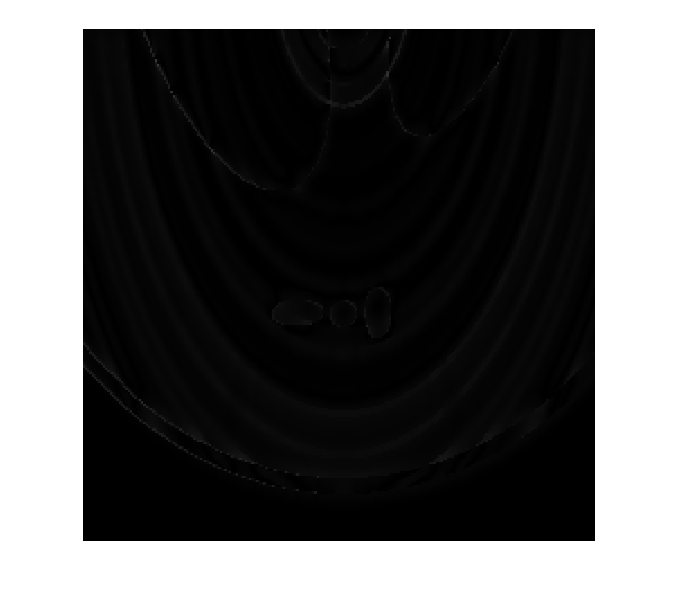
\includegraphics[scale=0.2]{4-2.png}
			}
			\quad
		\end{figure}
	
		\begin{multicols}{2}
			为了进一步探究图像损失对本文算法的影响,我们扩大了图像损失的的范围,它从原来的0.01增加到0.015.图* 是扩大之后的结果.对比(b)与(c)可以明显的看出最外层的伪影残留相对较为明显,所以这次我们选取的ROI为中心位置和边缘位置.对于(f)中心位置可以明显看出,在这个范围下,中心位置依然有很好的效果,同时对比中心像素边缘位置,锯齿结果基本没有发生变化.对于(i)这个ROI来说,该区域有一定的伪影残留,但绝大部分的伪影已经得到剔除.从表*可以看出相对与图像损失较小的情况,虽然PSNR,SSIM略微下降,但数据依然非常理想.
		\begin{tabular}{ccc}
			\hline
			\multirow{2}{*}{算法} & \multicolumn{2}{c}{Shepp-Logan 图像}  \\
			& SSIM             & PSNR                 \\ \hline
			1                  & 0.9550                & 49.814                \\
			2                & 0.9655                & 57.443                \\
			3               & 0.9685                & 58.6744                   \\ \hline
		\end{tabular}
		\end{multicols}
		
		
		
		\begin{figure}[H]
			\centering
			\subfigure[]{
				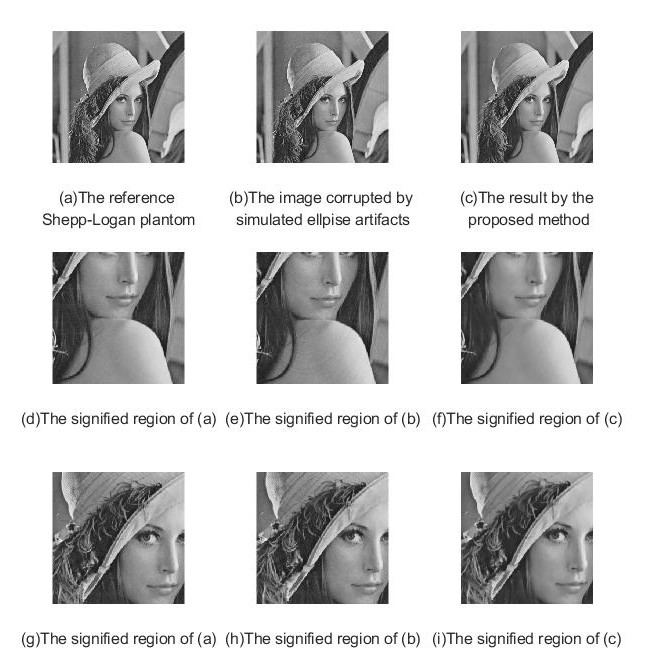
\includegraphics[scale=0.9]{test4}
				
			}
		\end{figure}
	
		\begin{multicols}{2}
		Using Lena phantom as our second stimulated data,(a),(b)and(c) are reference plantom, the image corrupted by simulated ellpise artifacts and  the proposed method.Although the image is quite different from CT image, the image not only contains a lot of details and textures, but also has smooth areas. In simulation experiment, it is of high significance to consider the processin results.从(a)~(c)组图像中,可以发现,(b)中的绝大部分的椭圆形伪影已得到处理,且图像(a)的主结构和纹理在图像(c)中没有发生明显的改变.为了观察跟细节的纹理,我们选取的两块区域,(d)~(f)为相对平滑的区域;(g)~(i)为细节较为复杂的区域.在(d)~(f)中可以观察到,伪影部分已经得到较为良好的处理,平滑区域未发生明显结构特征的改变.在(g)~(i)中伪影部分也基本得到较为良好的处理,且图像中"帽子绒毛"部分的细节没有发生明显的改变.
		
		\begin{tabular}{ccccc}
				\hline
				\multirow{2}{*}{算法} & \multicolumn{2}{c}{Shepp-Logan 图像} & \multicolumn{2}{c}{Lena图像} \\
				& PSNR             & SSIM            & PSNR         & SSIM        \\ \hline
				WF                  & 1                & 1               & 1            & 1           \\
				RCP                 & 1                & 1               & 1            & 1           \\
				VDM                 & 1                & 1               & 1            & 1           \\
				THIS                & 1                & 1               & 1            & 1           \\ \hline
		\end{tabular}
		\end{multicols}
	
		\begin{figure}[htbp]
			\centering
			\subfigure[pic1.]{
				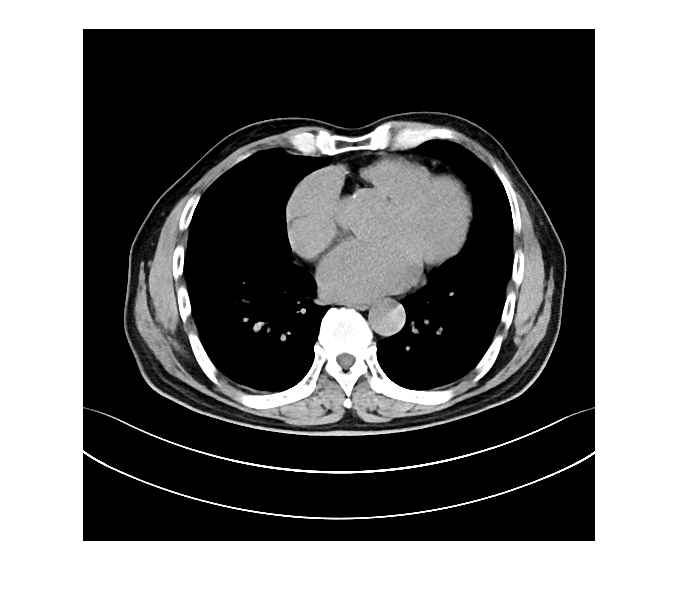
\includegraphics[scale=0.2]{111.png}
				%\caption{fig1}
			}
			\quad
			\subfigure[pic2.]{
				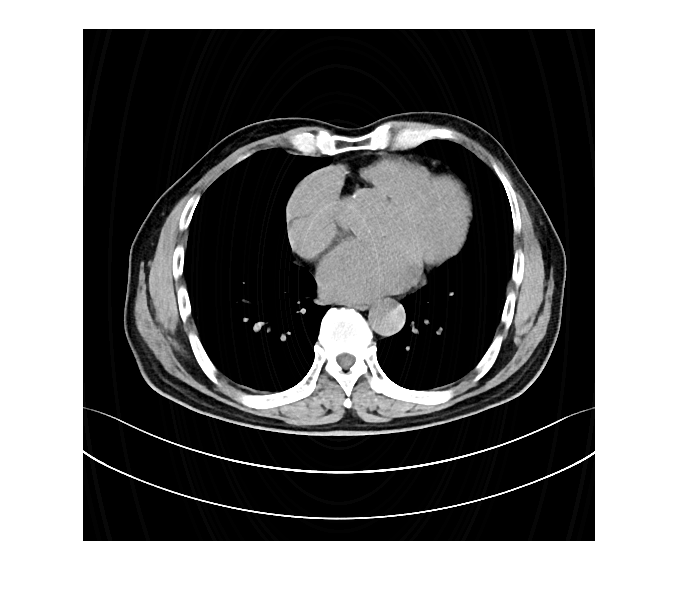
\includegraphics[scale=0.2]{222.png}
			}
			\quad
			\subfigure[pic3.]{
				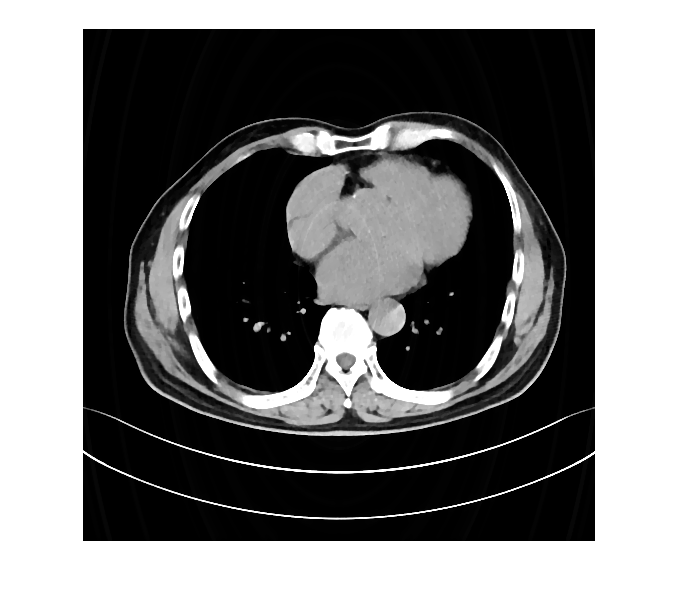
\includegraphics[scale=0.2]{333.png}
			}
			\quad
			\subfigure[pic4.]{
				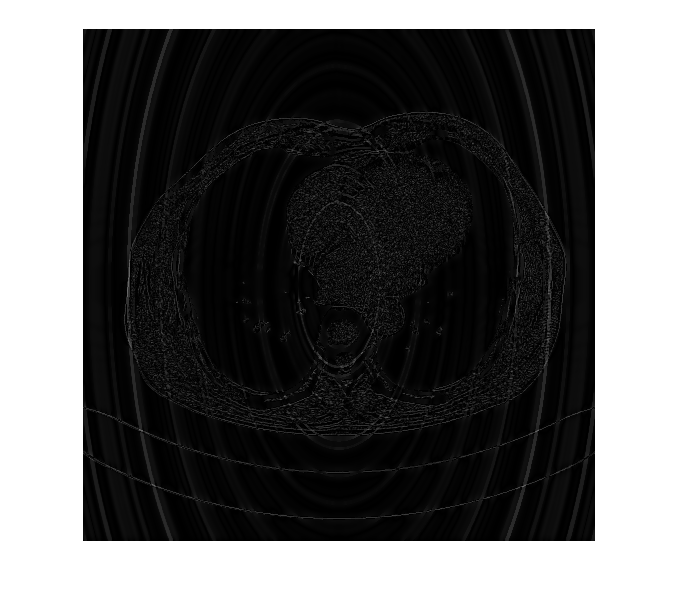
\includegraphics[scale=0.2]{444.png}
			}
			\quad
			\subfigure[pic5.]{
				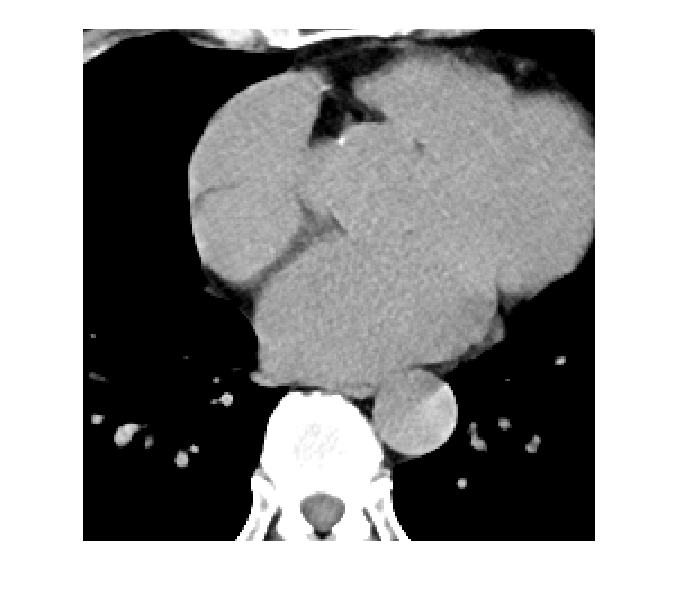
\includegraphics[scale=0.2]{111-1.png}
			}
			\quad
			\subfigure[pic6.]{
				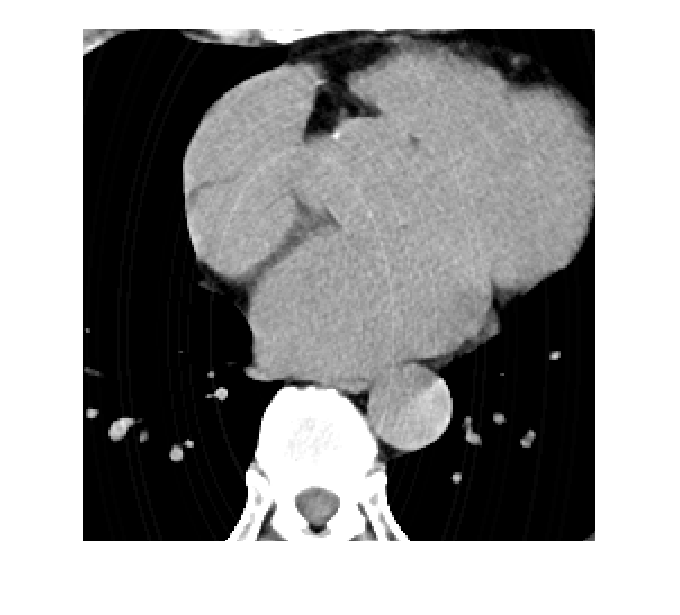
\includegraphics[scale=0.2]{222-1.png}
			}
			\quad
			\subfigure[pic1.]{
				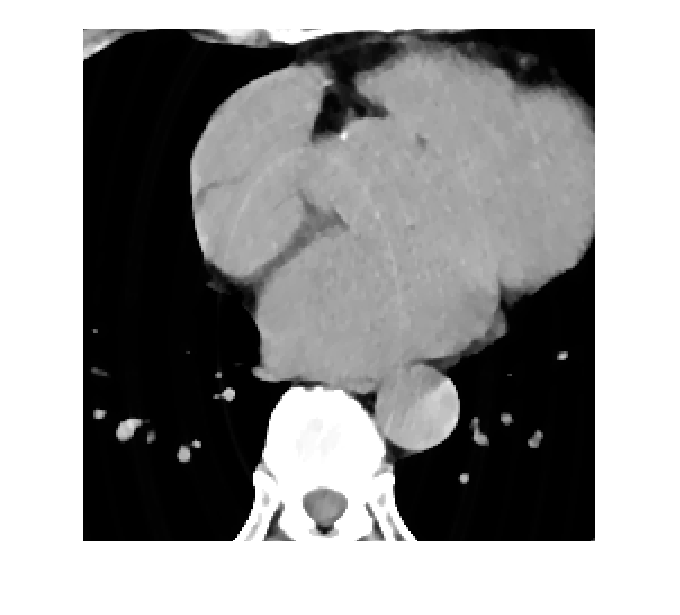
\includegraphics[scale=0.2]{333-1.png}
				%\caption{fig1}
			}
			\quad
			\subfigure[pic2.]{
				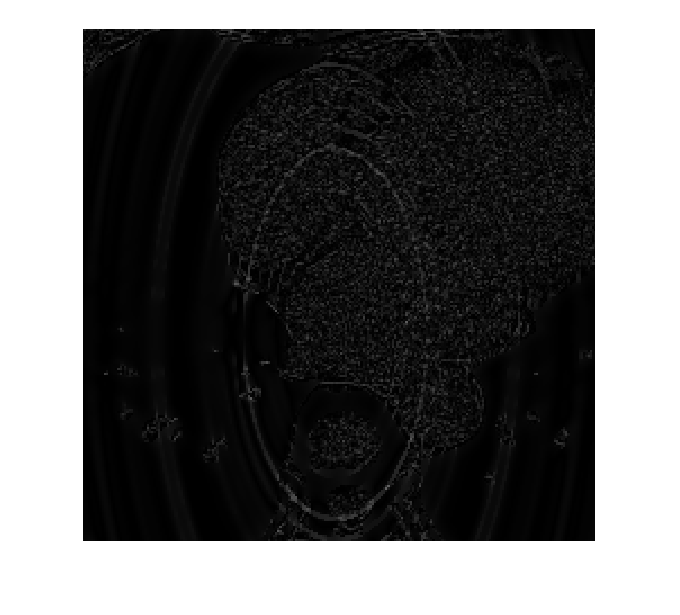
\includegraphics[scale=0.2]{444-1.png}
			}
			\quad
			\subfigure[pic5.]{
				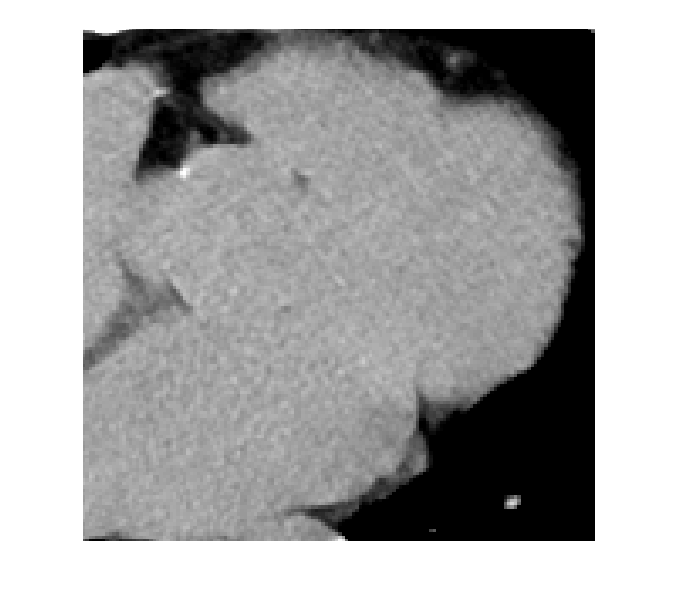
\includegraphics[scale=0.2]{111-2.png}
			}
			\quad
			\subfigure[pic6.]{
				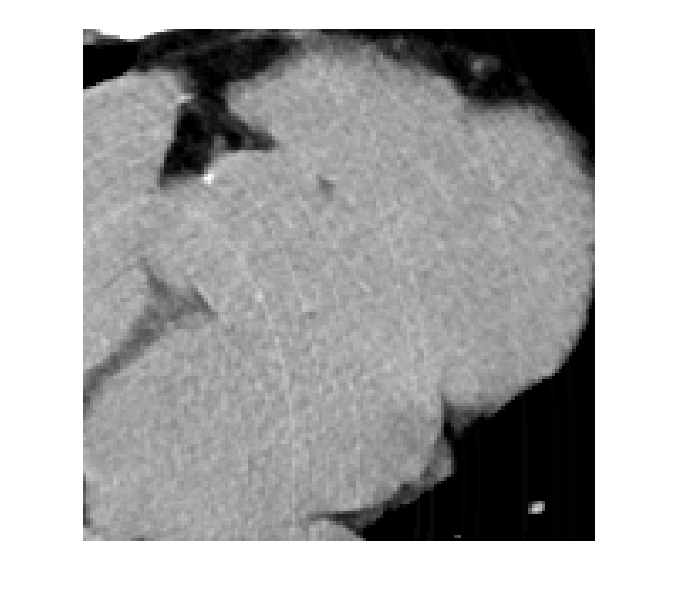
\includegraphics[scale=0.2]{222-2.png}
			}
			\quad
			\subfigure[pic1.]{
				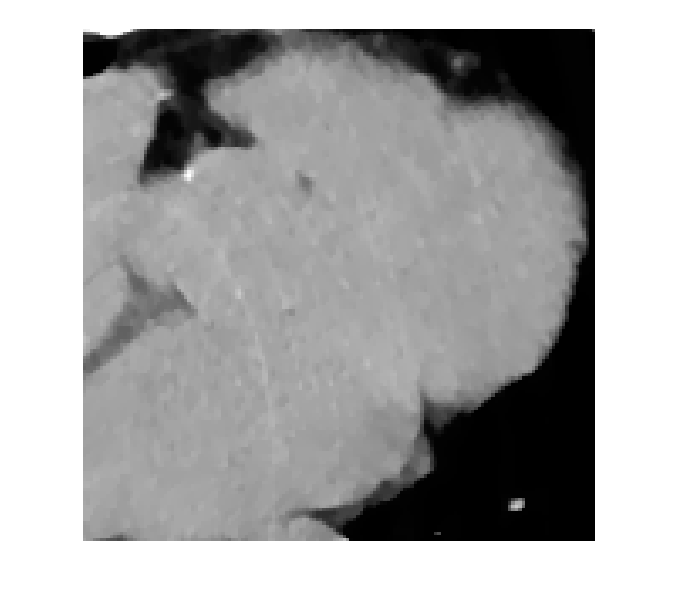
\includegraphics[scale=0.2]{333-2.png}
				%\caption{fig1}
			}
			\quad
			\subfigure[pic2.]{
				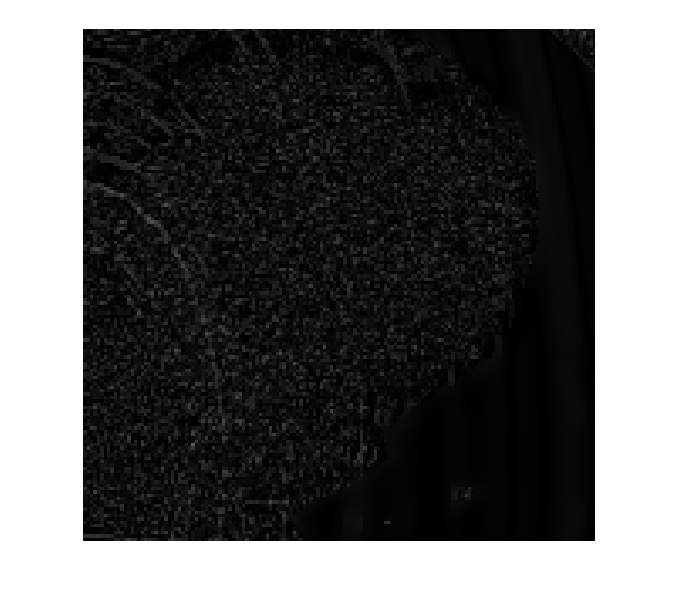
\includegraphics[scale=0.2]{444-2.png}
			}
			\quad
		\end{figure}
		
		\begin{multicols}{2}
			Using Lena phantom as our second stimulated data,(a),(b)and(c) are reference plantom, the image corrupted by simulated ellpise artifacts and  the proposed method.Although the image is quite different from CT image, the image not only contains a lot of details and textures, but also has smooth areas. In simulation experiment, it is of high significance to consider the processin results.从(a)~(c)组图像中,可以发现,(b)中的绝大部分的椭圆形伪影已得到处理,且图像(a)的主结构和纹理在图像(c)中没有发生明显的改变.为了观察跟细节的纹理,我们选取的两块区域,(d)~(f)为相对平滑的区域;(g)~(i)为细节较为复杂的区域.在(d)~(f)中可以观察到,伪影部分已经得到较为良好的处理,平滑区域未发生明显结构特征的改变.在(g)~(i)中伪影部分也基本得到较为良好的处理,且图像中"帽子绒毛"部分的细节没有发生明显的改变.
			
			\begin{tabular}{ccc}
				\hline
				\multirow{2}{*}{算法} & \multicolumn{2}{c}{Shepp-Logan 图像}  \\
				& SSIM             & PSNR                 \\ \hline
				1                  & 0.8631                & 39.1147              \\
				2                & 0.8381               & 39.1242                \\
				3               & 0.8921                & 40.8791                   \\ \hline
			\end{tabular}
		\end{multicols}
	
	
		\begin{figure}[htbp]
			\centering
			\subfigure[itteration of ssim]{
				\includegraphics[scale=0.5]{ssim.png}
				%\caption*{the title of figure}
				\label{fig:side:a}
			}
			\quad
			\subfigure[itteration of psnr]{
				\includegraphics[scale=0.5]{psnr.png}
			}
		\end{figure}
	
		\begin{multicols}{2}
		\section*{讨论}
			To investigate the practical convergence of our ETV algorithm, typical convergence curves (from the shepp-logan with gaussian, which sigma is 0.0018) are plotted in Fig * for both SSIM and RMSE. As we can see, the error decreases monotonically, and it remains stable after a few iterations. A similar trend can be observed from the psnr as it approaches to 82 after a few iterations and then remains stable. For future work, other improvements can be performed on the ETV algorithm.
		\end{multicols}
	
		\begin{multicols}{2}
		\section*{Acknowledgments}
		These are acknowledgments. These are acknowledgments. These are acknowledgments. These are acknowledgments. These are acknowledgments. These are acknowledgments.
		\begin{thebibliography}{100}%此处数字为最多可添加的参考文献数量
			\bibitem{article1}This is reference.%title author journal data pages
			\bibitem{book1}This is reference.%title author publish date
		\end{thebibliography}
	\end{multicols}
\end{document}